\lecture{Lecture - 14 \hfill 30 Sep 24, Mon}

\section{General Linear Recurrence Relations}

\begin{definition}[Linear Recurrence Relation]
	A \emph{recurrence relation,} or \emph{difference equation} is some relation constraining the elements of a sequence $\{ y_n \}_n.$
\end{definition}

A \emph{linear recurrence relation} on $\{ y_n \}$ is an equation
of the form 
$$ y_n = a_1 y_{n-1} + a_2 y_{n-2} + \cdots + a_k y_{n-k}.$$

\begin{remark}
	In order to find a recurrence relation involving $k$ terms, uniquely, we need
	initial conditions in the form of $k$ linearly independent
	equations, or equivalently, the first $k$ terms.
\end{remark}

Assuming that the $y_n$ is expressed by $x^n,$ for some each $n$ in 
$\mathbb{N},$ where $x$ is some value in $\mathbb{K},$
write the characteristic equation 
$$x^k = a_1 x^{k-1} + a_2 x^{k-2} + \cdots + a_{k-1} x + a_k.$$
Suppose the equation has $l$ distinct solutions $\alpha_1, \alpha_2,
\dotsc, \alpha_l,$ then any linear combination of these solutions:
$y^n = b_1 \alpha_1^n + b_2 \alpha_2^n + \cdots b_l \alpha_l^n$ is 
also a solution to the recurrence relation.
If the solutions $\alpha_1, \alpha_2, \dotsc, \alpha_l$ are not
distinct, and $\alpha_i$ is a solution of multiplicity $r$ where 
$r$ is some positive integer, then $\alpha_i^n, n \alpha_i^n, \dotsc,
n^{r-1} \alpha_i^n$ are all solutions of the recurrence relation.

\section{Catalan Numbers}
\begin{definition}[Curve]
	A \emph{curve} in a space $X$ is a continuous function $f \colon [0,1]
	\to X.$ 
\end{definition}
The points $f(0)$, respectively $f(1)$, as in the previous definition are known
as the starting point, respectively ending point, of $f.$
\begin{definition}[Simple Curve]
	A \emph{simple curve} is a continuous function $f \colon [0,1] \to X.$
	which is injective on $(0,1).$
\end{definition}
\begin{definition}[Closed curve]
	A \emph{closed curve} is a curve starting and ending at the same
	point.
\end{definition}
\begin{definition}[Jordan Curve]
	A Jordan curve is a simple closed curve in the plane $\mathbb{R}.$	
\end{definition}
\begin{theorem}[Jordan Curve Theorem]
	If $c$ is a Jordan curve in $\mathbb{R}^2$ then $\mathbb{R}^2
	\setminus \operatorname{Image}(c)$ consists of exactly 2 
	connected components, one bounded, called the `interior of $c$',	and one unbounded,
	called the `exterior of $c.$' The boundary of both of these connected components is $\operatorname{image}(c).$
\end{theorem}

\begin{definition}[Polygon]
	A polygon is a Jordan curve which is piecewise linear.
\end{definition}
\begin{definition}[Convex polygon]
	A convex polygon is a polygon whose interior is a convex set in
	$\mathbb{R}^2.$
\end{definition}

\begin{center}
	\incfig{polygons}{0.4}
\end{center}


\begin{figure}[h]
\centering
	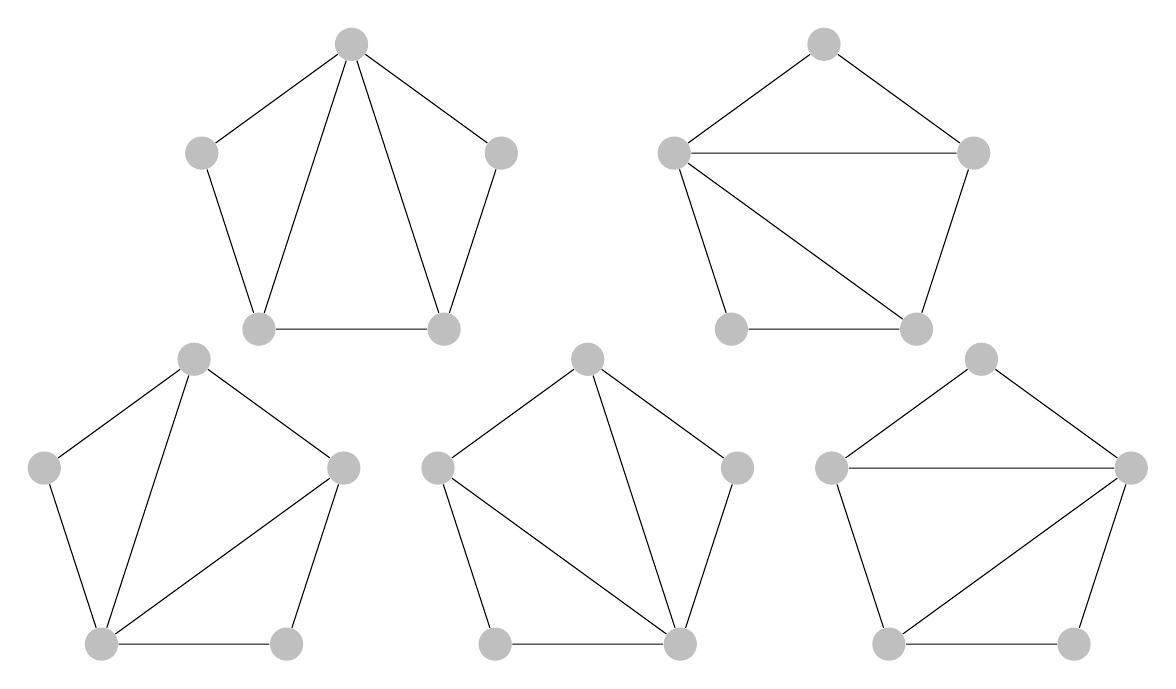
\begin{tikzpicture}
		\tikzstyle{vertex}=[circle,fill=black!25,minimum size=12pt,inner sep=2pt]
	shift={(3,4)}
	\newcommand*{\coords}{\foreach \x in {1,...,5}{
		\node[vertex] (g_\x) at (18+72*\x:2) {};
}}
	\begin{scope}[shift={(-3,4)}]
		\coords
		\draw (g_1) -- (g_2) -- (g_3) -- (g_4) -- (g_5) -- (g_1) (g_1) -- (g_3) (g_1) -- (g_4);
	\end{scope}
	\begin{scope}[shift={(3,4)}]
		\coords
		\draw (g_1) -- (g_2) -- (g_3) -- (g_4) -- (g_5) -- (g_1)(g_2) -- (g_5) (g_2) -- (g_4); 
	\end{scope}
	\begin{scope}[shift={(-5,0)}]
		\coords
		\draw (g_1) -- (g_2) -- (g_3) -- (g_4) -- (g_5) -- (g_1) (g_3) -- (g_1) (g_3) -- (g_5);
	\end{scope}
	\begin{scope}[shift={(0,0)}]
		\coords
		\draw (g_1) -- (g_2) -- (g_3) -- (g_4) -- (g_5) -- (g_1) (g_4) -- (g_2) (g_4) -- (g_1);
	\end{scope}
	\begin{scope}[shift={(5,0)}]
		\coords
		\draw (g_1) -- (g_2) -- (g_3) -- (g_4) -- (g_5) -- (g_1) (g_5) -- (g_3) (g_5) -- (g_2);
	\end{scope}
	\end{tikzpicture}
	\caption{Triangulations of a pentagon}
\end{figure}

$C_2 = 2,$ $C_3 = 5,$ $C_4 = 14,$ $C_5 = 42,$ $C_6 = 132,$ $C_7 = 429,$
$C_8 = 1430.$
